\def\scale{0.315}
\def\dir{exp1/ver1/examples/output}
\def\imgwidth{0.3\textwidth}
\def\hspacebase{\hspace{-1.5em}}
\def\vspacebase{\vspace{0.5em}}
\def\vspacebeforecaption{\vspace{-0.4em}}

\newcommand{\limesubfigure}[2]{
	\begin{subfigure}[t]{\textwidth}
		\hspace{#2}
		\includegraphics[scale=\scale]{exp1/ver1/examples/output/lime-\sampleindex{#1}}
		\caption{LIME}\label{fig:lime-#1}
		\vspace{1.0em}
	\end{subfigure}
}
\newcommand{\anchorsubfigure}[1]{
	\foreach{\a} in {70,80,90}{
			\begin{subfigure}[t]{\textwidth}
				\centering
				\includegraphics[scale=0.33]{exp1/ver2/examples/anchor-\sampleindex{#1}-\a}
				\caption{\hl{Anchor ($\tau=0.\a$)}}
				\vspace{1.0em}
			\end{subfigure}
		}
}
\newcommand{\rlimesubfigure}[3]{
}
\begin{figure}[t]
	\begin{subfigure}[t]{0.45\textwidth}
		\centering
		\begin{subfigure}[t]{\textwidth}
			\hspace{-10pt}
			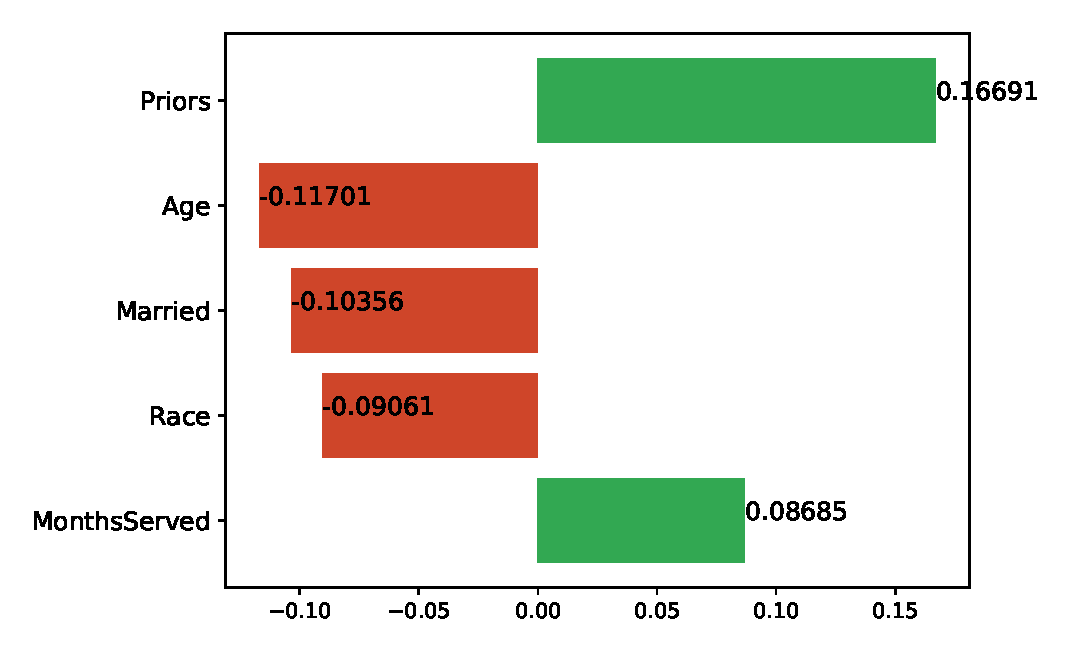
\includegraphics[scale=\scale]{exp1/ver1/examples/output/lime-0012}
			\caption{LIME}\label{fig:lime-0}
			\vspace{1.0em}
		\end{subfigure}

		\vspace{10pt}
		\begin{subfigure}[t]{\textwidth}
			\centering
			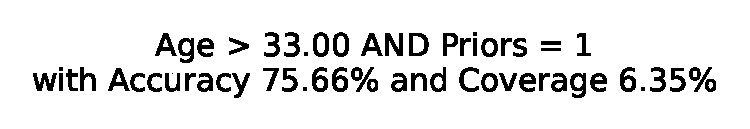
\includegraphics[scale=0.33]{exp1/ver2/examples/anchor-0012-70}  % chktex 8
			\caption{\hl{Anchor ($\tau=0.70$)}}\label{fig:anchor-0-70}
			\vspace{1.0em}
		\end{subfigure}

		\vspace{10pt}
		\begin{subfigure}[t]{\textwidth}
			\centering
			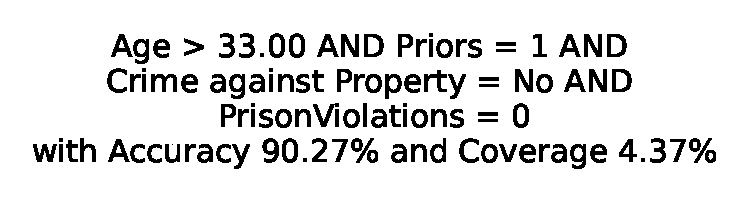
\includegraphics[scale=0.33]{exp1/ver2/examples/anchor-0012-90}  % chktex 8
			\caption{\hl{Anchor ($\tau=0.90$)}}\label{fig:anchor-0-90}
			\vspace{1.0em}
		\end{subfigure}
	\end{subfigure}
	\hfill
	\begin{subfigure}[t]{0.45\textwidth}
		\begin{subfigure}[t]{\textwidth}
			\hspacebase{}
			\hspace{-5pt}
			\includegraphics[scale=\scale]{exp1/ver1/examples/output/newlime-0012-70}  % chktex 8
			\vspacebeforecaption{}
			\caption{R-LIME ($\tau=0.70$)}\label{fig:rlime-0-70}
			\vspacebase{}
		\end{subfigure}
		\begin{subfigure}[t]{\textwidth}
			\hspacebase{}
			\hspace{-17pt}
			\includegraphics[scale=\scale]{exp1/ver1/examples/output/newlime-0012-90}  % chktex 8
			\vspacebeforecaption{}
			\caption{R-LIME ($\tau=0.90$)}
			\vspacebase{}
		\end{subfigure}
	\end{subfigure}
	\caption[Explanation for Instance A by LIME and R-LIME]{%
		Explanation for Instance A by LIME and R-LIME\@.
	}\label{fig:A}
\end{figure}
\begin{figure}[t]
	\begin{subfigure}[t]{0.45\textwidth}
		\begin{subfigure}[t]{\textwidth}
			\hspace{-26.5pt}
			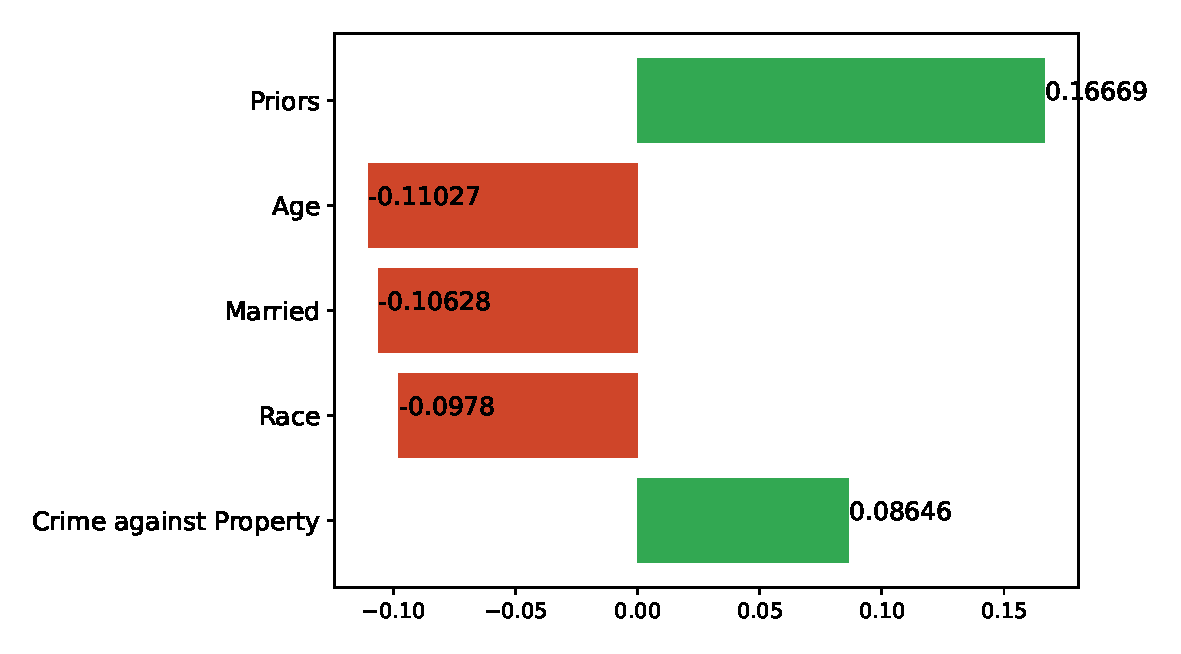
\includegraphics[scale=\scale]{exp1/ver1/examples/output/lime-0011}
			\caption{LIME}\label{fig:lime-1}
			\vspace{1.0em}
		\end{subfigure}

		\vspace{10pt}
		\begin{subfigure}[t]{\textwidth}
			\centering
			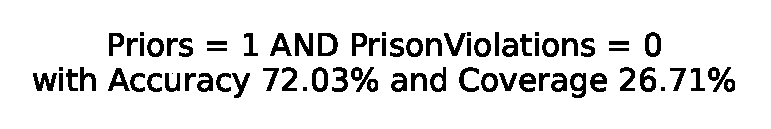
\includegraphics[scale=0.33]{exp1/ver2/examples/anchor-0011-70}  % chktex 8
			\caption{\hl{Anchor ($\tau=0.70$)}}\label{fig:anchor-1-70}
			\vspace{1.0em}
		\end{subfigure}

		\vspace{10pt}
		\begin{subfigure}[t]{\textwidth}
			\centering
			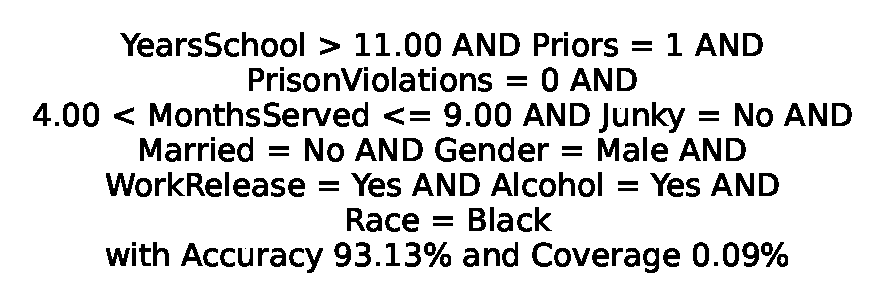
\includegraphics[scale=0.33]{exp1/ver2/examples/anchor-0011-90}  % chktex 8
			\caption{\hl{Anchor ($\tau=0.90$)}}\label{fig:anchor-1-90}
			\vspace{1.0em}
		\end{subfigure}
	\end{subfigure}
	\hfill
	\begin{subfigure}[t]{0.45\textwidth}
		\begin{subfigure}[t]{\textwidth}
			\hspacebase{}
			\hspace{-5pt}
			\includegraphics[scale=\scale]{exp1/ver1/examples/output/newlime-0011-70}  % chktex 8
			\vspacebeforecaption{}
			\caption{R-LIME ($\tau=0.90$)}
			\vspacebase{}
		\end{subfigure}
		\begin{subfigure}[t]{\textwidth}
			\hspacebase{}
			\hspace{-20pt}
			\includegraphics[scale=\scale]{exp1/ver1/examples/output/newlime-0011-90}  % chktex 8
			\vspacebeforecaption{}
			\caption{R-LIME ($\tau=0.90$)}\label{fig:rlime-1-90}
			\vspacebase{}
		\end{subfigure}
	\end{subfigure}
	\caption[Explanation for Instance B by LIME and R-LIME]{%
		Explanation for Instance B by LIME and R-LIME\@.
	}\label{fig:B}
\end{figure}
